\documentclass{beamer}

%%%%%%%%%%%%%Solarized Theme%%%%%%%%%%%%%%%
\usecolortheme[dark,accent=cyan]{solarized}
\beamertemplatenavigationsymbolsempty

%%%%%Packages%%%%%
\usepackage{graphicx}
\usepackage{hyperref}
\usepackage{colortbl, xcolor}
\usepackage{booktabs}

\usepackage{tikz}
\usepackage{standalone}
\usetikzlibrary{calc}

\usepackage{color}

\usetikzlibrary{decorations.pathmorphing}
\usetikzlibrary{fit}                    % fitting shapes to coordinates
\usetikzlibrary{backgrounds}    % drawing the background after the foreground

\tikzstyle{background}=[red, rectangle, draw, inner sep=-0.5mm,
           rounded corners=1mm]
\usepackage{minted}

\definecolor{DarkGray}{gray}{0.1}
\definecolor{DarkGray}{gray}{0.1}
\usemintedstyle{native}

%%%%%%Title%%%%%%%%
\title{Machine Learning and the Iterated Prisoner's Dilemma}
\author{@NikoletaGlyn}
\date{\small{\textit{Supervised by:}} \\ Dr. Vincent \textsc{Knight}}
\institute[]
{
% \begin{center}
%     
\includegraphics[width=.20\textwidth]{cardiff_uni_logo.jpg}
% \end{center}
}
\begin{document}

\maketitle  

% \begin{frame}
%     \begin{columns}[T] % align columns
%     \begin{column}{.515\textwidth}
%          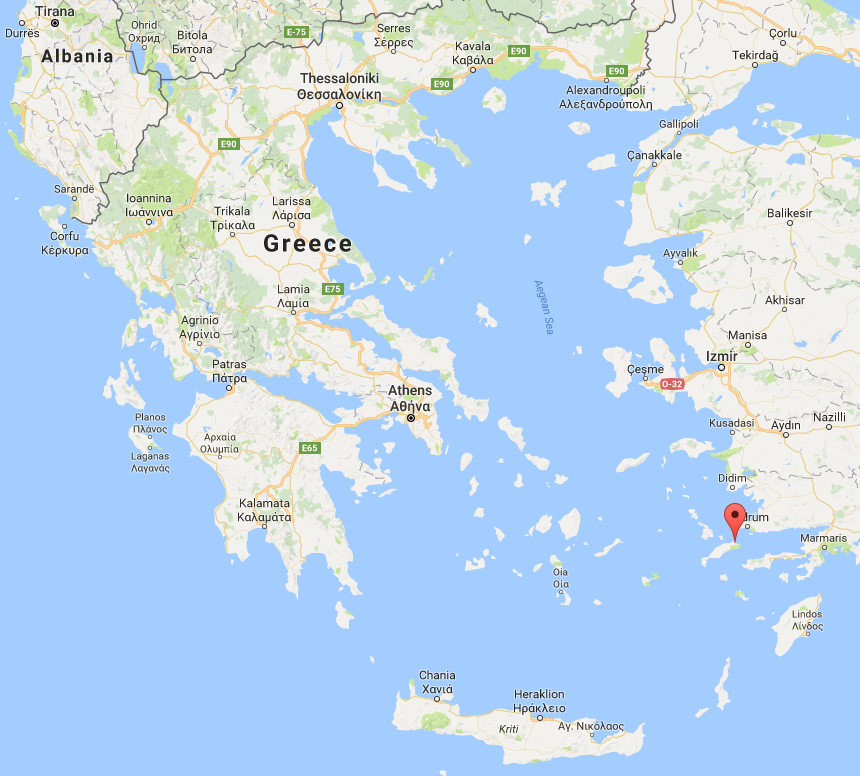
\includegraphics[width=\textwidth]{static/kos.png}
%     \end{column}% 
%     \begin{column}{.23\textwidth}
%         
\includegraphics[width=\textwidth]{static/cardiff_uni_logo.jpg}

%         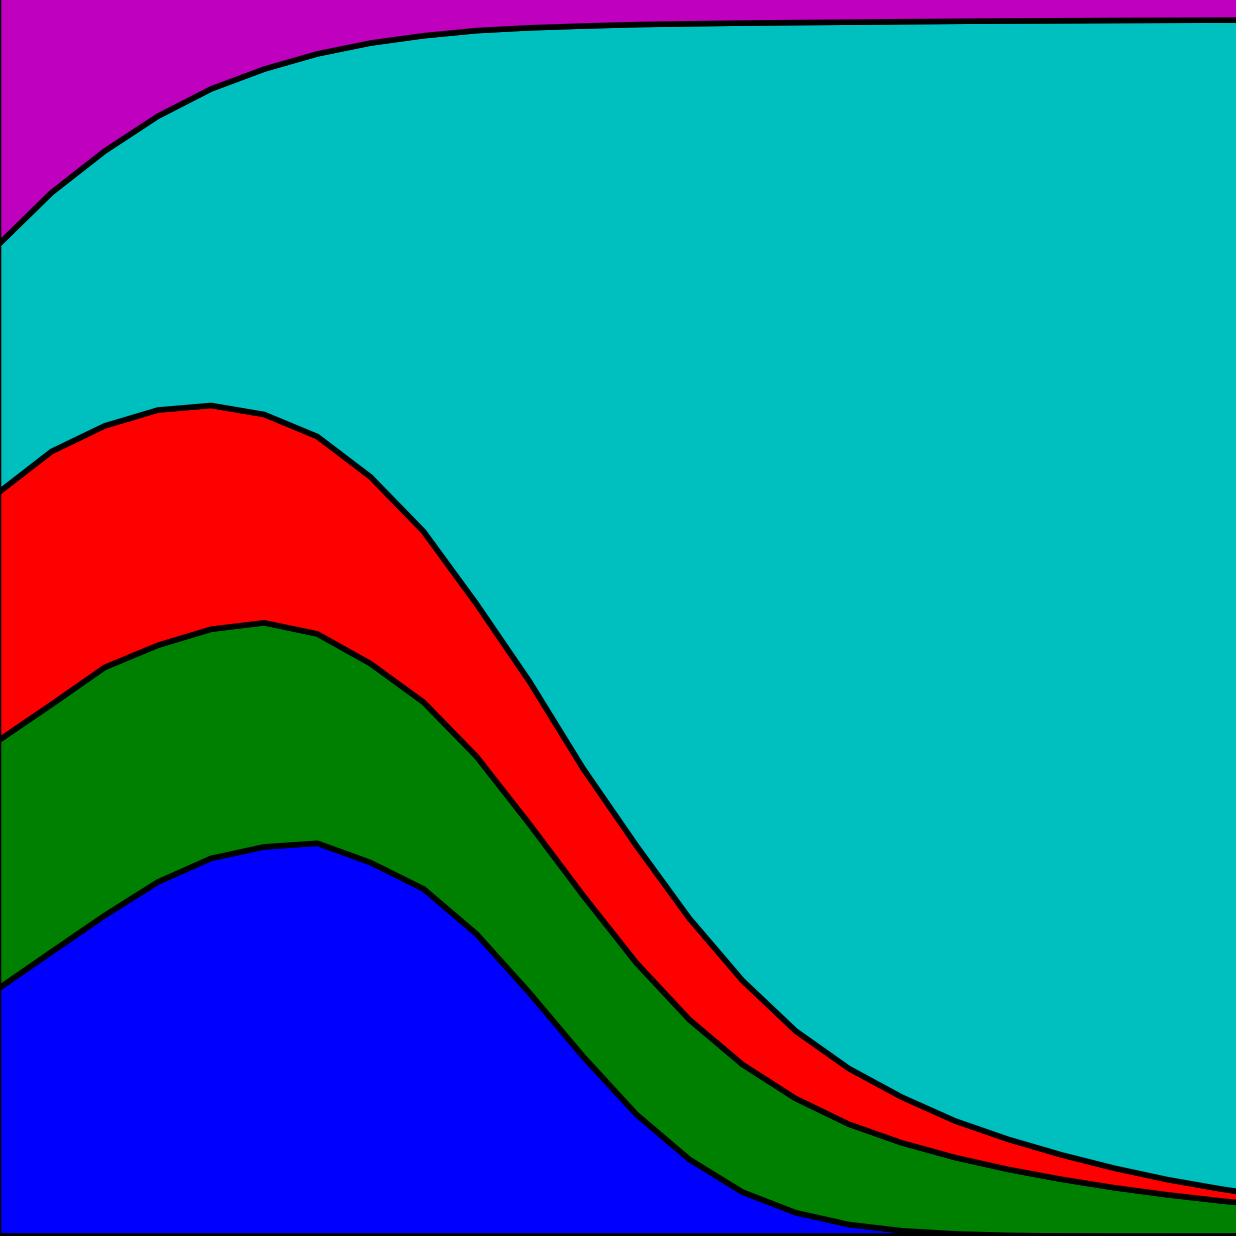
\includegraphics[width=\textwidth]{static/axelrod-logo.png}
%     \end{column}%
%     \begin{column}{.23\textwidth}
%         
\includegraphics[width=\textwidth]{static/ssi-logo.png}

%         
\includegraphics[width=\textwidth]{static/phoenix-logo.jpg}
% \end{column}%
% \end{columns}
% \end{frame}

% A frame to explain the IPD

\begin{frame}
\begin{center}
    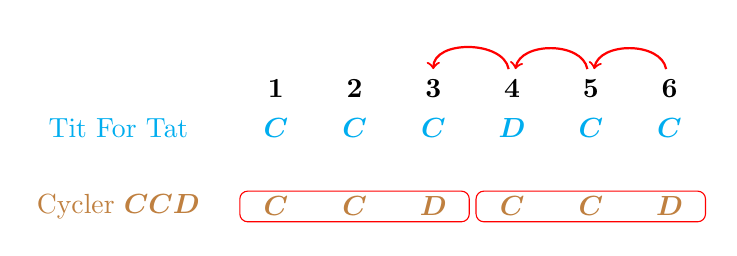
\begin{tikzpicture}

    \tikzstyle{state}=[minimum width=1cm, font=\boldmath];
    

    \node[thick] (0) at (-1, 0) [state] {\textcolor{cyan}{Tit For Tat}};
    \node[thick] (1) at (-1, -1) [state] {\textcolor{brown}{Cycler $CCD$}};
    \pause

    \node[thick] (2) at (1, 0.5) [state] {$1$};
    \node (8) at (1, 0) [state] {\textcolor{cyan}{$C$}};
    \node (14) at (1, -1) [state] {\textcolor{brown}{$C$}};   
    
    \pause

    \node[thick] (3) at (2, 0.5) [state] {$2$};
    \node[thick] (4) at (3, 0.5) [state] {$3$};
    \node (9) at (2, 0) [state] {\textcolor{cyan}{$C$}};
    \node (10) at (3, 0) [state] {\textcolor{cyan}{$C$}};
    \node (15) at (2, -1) [state] {\textcolor{brown}{$C$}};
    \node (16) at (3, -1) [state] {\textcolor{brown}{$D$}};

    \pause
    \node [background, fit=(14) (15) (16)] {};
    \pause
    \node[thick] (5) at (4, 0.5) [state] {$4$};
    \draw (5) edge[red, out=100, in=90, ->, thick] node [above] {} (4);

    \pause
    \node (11) at (4, 0) [state] {\textcolor{cyan}{$D$}};
    \node (17) at (4, -1) [state] {\textcolor{brown}{$C$}};

    \pause
    \node[thick] (6) at (5, 0.5) [state] {$5$};
    \node[thick] (7) at (6, 0.5) [state] {$6$};

    \node (12) at (5, 0) [state] {\textcolor{cyan}{$C$}};
    \node (13) at (6, 0) [state] {\textcolor{cyan}{$C$}};

    \node (18) at (5, -1) [state] {\textcolor{brown}{$C$}};
    \node (19) at (6, -1) [state] {\textcolor{brown}{$D$}};


    \draw (6) edge[red, out=100, in=80, ->, thick] node [above] {} (5);
    \draw (7) edge[red, out=100, in=80, ->, thick] node [above] {} (6);

    \node [background, fit=(17) (18) (19)] {};

    \end{tikzpicture}
\end{center}
\end{frame}

\begin{frame}
    \begin{center}
        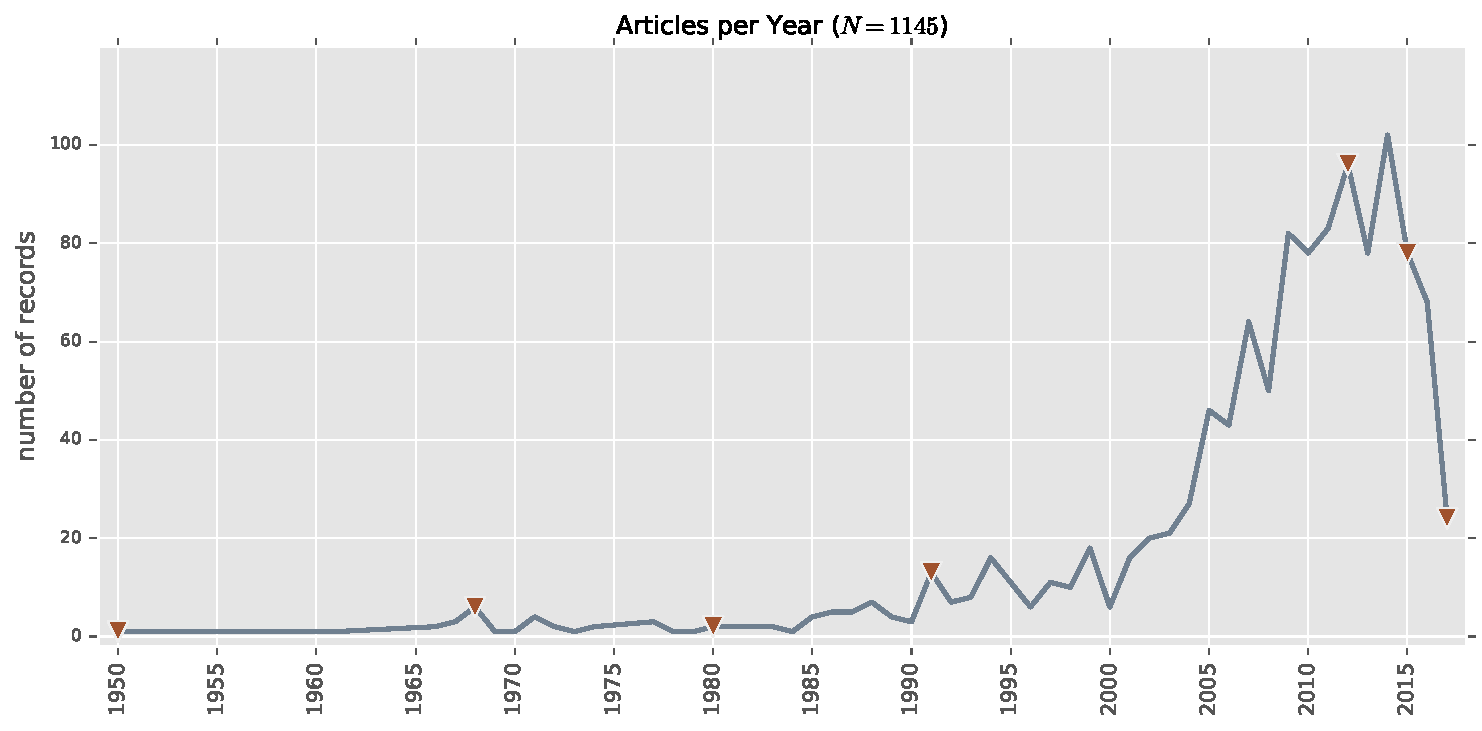
\includegraphics[width=\textwidth]{static/timeline.pdf}
    \end{center}
\end{frame}

\begin{frame}
    \begin{center}
        
\includegraphics[width=0.8\textwidth]{static/death_star.png}
    \end{center}
\end{frame}

\begin{frame}
\begin{columns}[T] % align columns
    \begin{column}{.5\textwidth}
        
\includegraphics[width=\textwidth]{static/shell.png}

        \end{column}% 
    \begin{column}{.6\textwidth}
        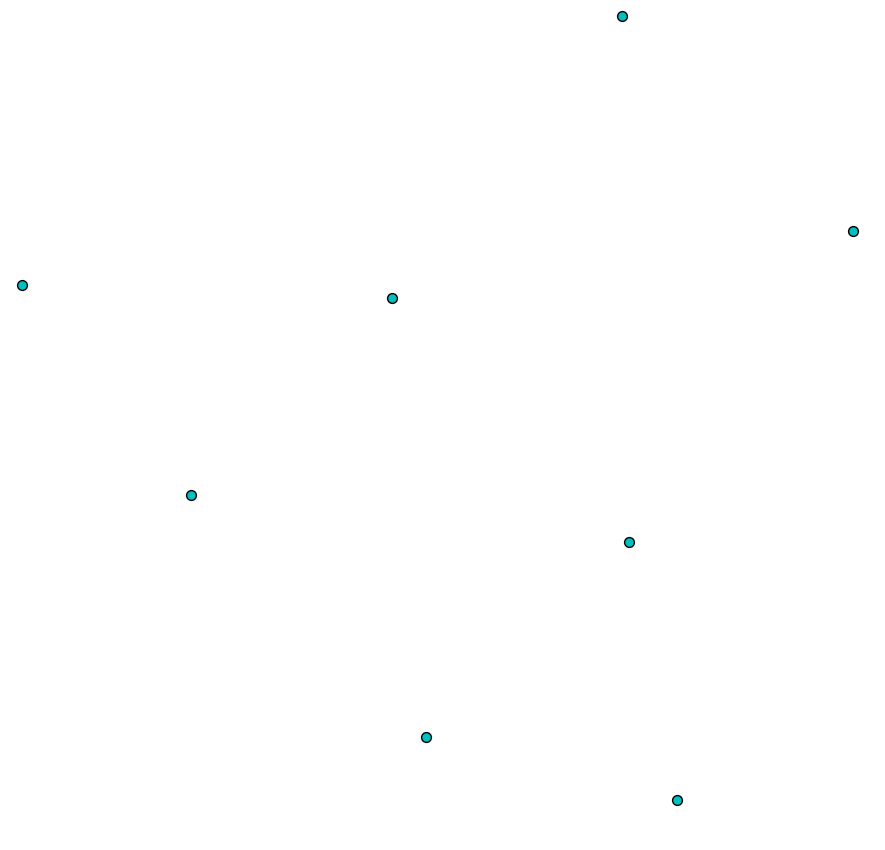
\includegraphics[width=\textwidth]{static/sedgewick.png}

       \vspace{-3cm} 
       \hspace{-2cm} 
\includegraphics[width=\textwidth]{static/diamond.png}
    \end{column}
\end{columns}
\end{frame}

\begin{frame}
\begin{center}
    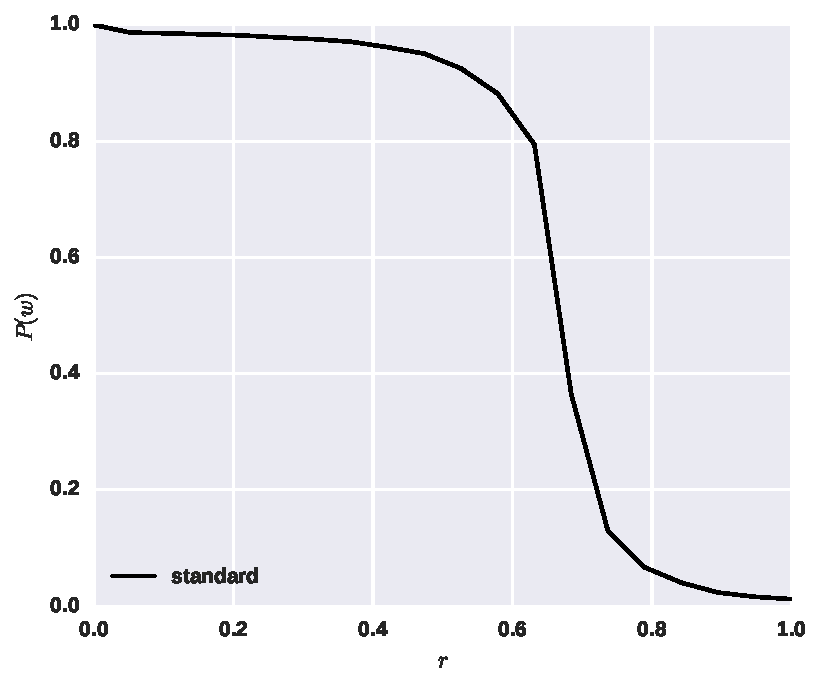
\includegraphics[width=0.48\textwidth]{static/standard.pdf}
    \hfill
    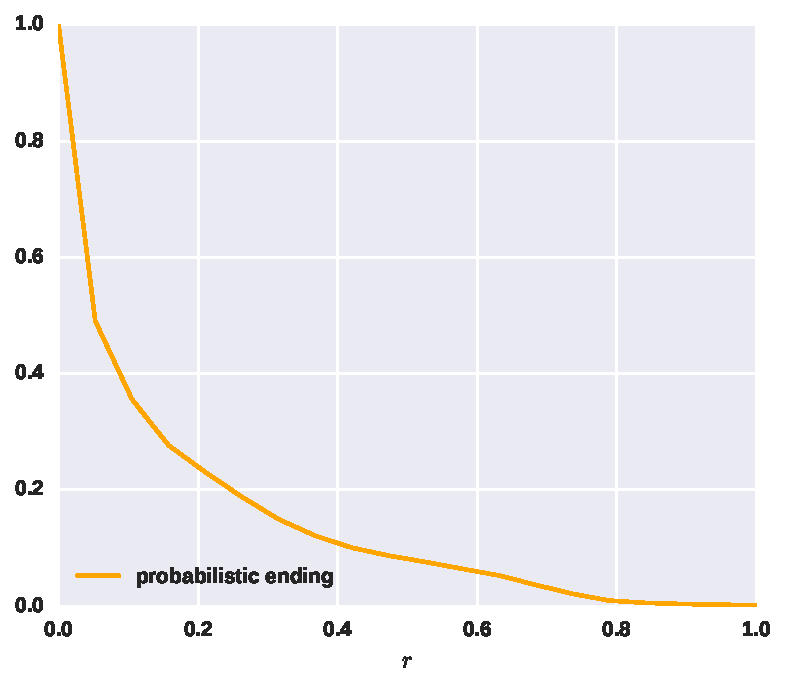
\includegraphics[width=0.48\textwidth]{static/probend.pdf}
\end{center}
\end{frame}

\begin{frame}
\begin{center}
    \includestandalone[width=0.6\textwidth]{static/memory_one_chain}
\end{center}
\end{frame}

\begin{frame}
    \begin{center}
       \begin{itemize}
        \item \textit{William Press and Freeman Dyson.} Iterated Prisoner’s
        Dilemma contains strategies that dominate any evolutionary opponent. 2012.
        \item  \textit{Christopher Lee, Marc Harper, and Dashiell Fryer.}
               The art of war: Beyond memory-one strategies in population games. 2015.
        \end{itemize}
    \end{center}
\end{frame}

\begin{frame}
    \begin{center}
        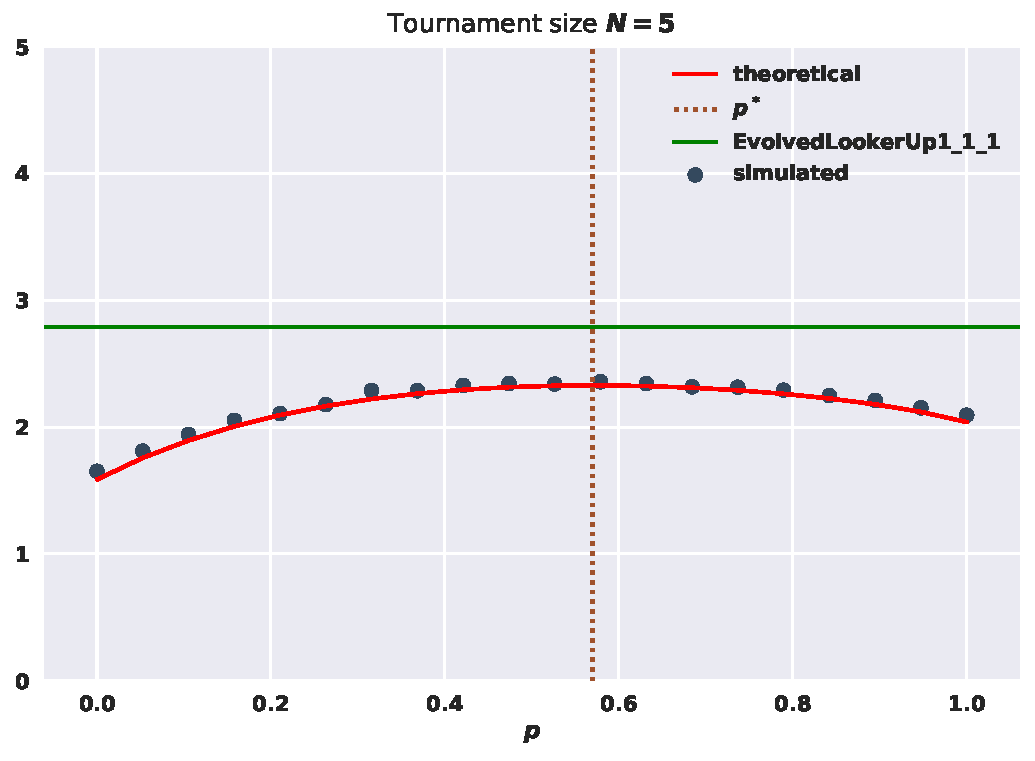
\includegraphics[width=0.8\textwidth]{static/optimisation.pdf}
    \end{center}
\end{frame}


\begin{frame}
    \begin{center}
        
\includegraphics[width=0.8\textwidth]{static/death_star.png}
    \end{center}
\end{frame}

\begin{frame}
    \begin{center}
        
\includegraphics[width=0.8\textwidth]{static/complex.png}
    \end{center}
\end{frame}

\end{document}

